
%(BEGIN_QUESTION)
% Copyright 2006, Tony R. Kuphaldt, released under the Creative Commons Attribution License (v 1.0)
% This means you may do almost anything with this work of mine, so long as you give me proper credit

Hvor stort trykk, i tommer vannsøyle, pålegges dette skra vannmanometeret for å gi en total forskyvning på 14 tommer langs rorlengdene, når rørene har vinkel 20$^{o}$ fra horisontalen?  Anta at bunnen av dette manometeret er plassert 24 tommer over bakkeniva.

$$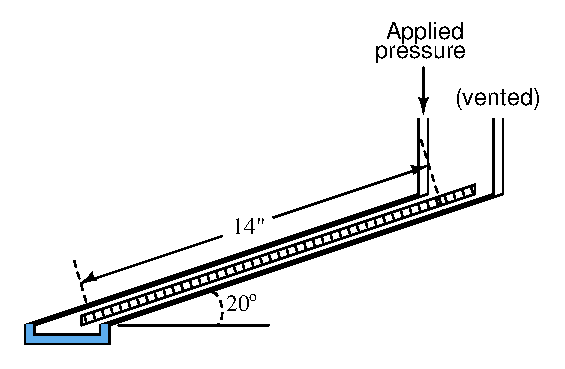
\includegraphics[width=15.5cm]{i00168x01.eps}$$

Konverter deretter dette trykket til kPa.

\vskip 20pt \vbox{\hrule \hbox{\strut \vrule{} {\bf Suggestions for Socratic discussion} \vrule} \hrule}

\begin{itemize}
\item{} Identifiser hvilke grunnleggende prinsipper fra naturfag, teknologi og/eller matematikk som gjelder i hvert steg av løsningen din.  Vaer med andre ord forberedt på å forklare ``hvorfor'' for hvert steg, ikke bare beskrive stegene.
\item{} Gjor skrastilling av et manometer det mer eller mindre følsomt for pålagt trykk?  Lag et ``tankeeksperiment'' der du kunne teste et manometer for å svare på dette.
\item{} Er det mulig å lage en \textit{brønn}-variant av et skrastilt manometer slik at vi bare trenger å lese av en væskesøyle?
\item{} Hva vil skje med et manometer hvis det utsettes for et gasstrykk som er større enn måleområdet?
\item{} Ville et \textit{mikromanometer} være mer eller mindre følsomt for pålagt trykk enn dette skrastilte manometeret?
\end{itemize}

\underbar{file i00168}
%(END_QUESTION)





%(BEGIN_ANSWER)

Pålagt trykk = 1.193 kPa

%(END_ANSWER)





%(BEGIN_NOTES)

Hoyden på 24 tommer over bakkeniva er overflødig informasjon, inkludert for å utfordre studenter til å avgjøre om informasjon er relevant for løsning av en bestemt oppgave.

\vskip 10pt

Den diagonale forskyvningen på 14 tommer tilsvarer bare en vertikal forskyvning på 4.7883 tommer, slik sinusfunksjonen beskriver:

$${h \over 14} = \sin 20$$

$$h = 14 \sin 20$$

$$h = 4.7883$$

Derfor er pålagt trykk lik 4.7883 tommer vannsøyle ("W.C).

\vskip 10pt

A tilnaerme visse trigonometriske funksjoner fra hukommelsen er ikke så vanskelig som man kanskje tror.  Se følgende ``enkle vinkler'' for sinus- og cosinusfunksjonene:

$$\sin 0^o = 0 = \cos 90^o$$

$$\sin 30^o = 0.5 = \cos 60^o$$

$$\sin 45^o = {\sqrt{2} \over 2} = \cos 45^o$$

$$\sin 60^o = {\sqrt{3} \over 2} = \cos 30^o$$

$$\sin 90^o = 1 = \cos 0^o$$

Disse kan bli enda enklere å huske ved å skrive konstantene litt annerledes:

$$\sin 0^o = {\sqrt{0} \over 2} = \cos 90^o$$

$$\sin 30^o = {\sqrt{1} \over 2} = \cos 60^o$$

$$\sin 45^o = {\sqrt{2} \over 2} = \cos 45^o$$

$$\sin 60^o = {\sqrt{3} \over 2} = \cos 30^o$$

$$\sin 90^o = {\sqrt{4} \over 2} = \cos 0^o$$

Mye enklere, ikke sant?

%INDEX% Measurement, pressure: inclined manometer
%INDEX% Mathematics, trigonometry: approximating trig functions from memory

%(END_NOTES)

